\documentclass[conference,10pt,letterpaper]{IEEEtran}
\usepackage{amsmath,amssymb,graphicx,booktabs,algorithm,algorithmic,tikz,pgfplots,xcolor,hyperref}
\usetikzlibrary{arrows.meta,positioning,calc,decorations.pathreplacing,shapes.geometric,fit}
\pgfplotsset{compat=1.18}

\title{AgentInfer: Autonomous AI Agents for 24/7\\Infrastructure Operations and Revenue Optimization\\in Distributed Inference Platforms}
\author{\IEEEauthorblockN{Srikanta Datta Tumkur*, Mehar Simhadri$^\dagger$, Jay Iyer$^\dagger$, Anshu Bansal*}
\IEEEauthorblockA{*MIT Sloan School of Management, Cambridge, MA \{srikanta, anshu.bansal\}@sloan.mit.edu\\$^\dagger$IEEE Senior Members \{mehar.simhadri, jay.iyer\}@ieee.org}}
\begin{document}
\maketitle

\begin{abstract}
Modern AI inference platforms require continuous, intelligent management across both infrastructure operations and customer-facing revenue functions. We present \textbf{AgentInfer}, an agentic AI framework that deploys autonomous LLM-powered agents for 24/7 infrastructure operations (NOC automation, incident response, capacity planning) and sales optimization (lead qualification, deal acceleration, customer success). AgentInfer integrates with our previously published control plane stack: InferMark observability (Paper~1), confidential multi-tenant isolation (Paper~3), InferTwin digital twins (Paper~4), VoxOps voice interface (Paper~5), hierarchical RL optimization (Paper~6), ReliableInfer fault tolerance (Paper~7), and SolarInfer edge deployment (Paper~8). Our key contributions include: (1)~a \emph{multi-agent orchestration} architecture with specialized Ops and Sales agent teams coordinated by a meta-agent planner; (2)~\emph{ReAct-based reasoning} with tool-use capabilities spanning 47 infrastructure APIs and 23 CRM integrations; (3)~\emph{RL-refined agent policies} that improve autonomously through Reflexion-style verbal reinforcement learning; (4)~\emph{confidential agent execution} via AMD SEV-SNP ensuring customer data isolation during multi-tenant agent operations; and (5)~a \emph{RAG-powered knowledge base} with 2.4M tokens of operational runbooks and sales playbooks. Deployed across a 500-node heterogeneous fleet, AgentInfer resolves 87\% of Sev-2+ incidents autonomously (MTTR: 4.2 min vs.\ 47 min human baseline), generates \$2.8M incremental ARR through automated lead nurturing, and operates at \$0.003 per agent action---94\% cheaper than equivalent human staffing.

\emph{Index Terms}---Agentic AI, autonomous operations, LLM agents, multi-agent systems, sales automation, inference infrastructure, reinforcement learning, RAG
\end{abstract}

\section{Introduction}
\label{sec:intro}

The operational complexity of distributed AI inference platforms has outpaced human capacity for 24/7 management. A production fleet spanning hundreds of heterogeneous nodes across multiple edge sites generates over 15,000 metrics per second, processes 200+ customer requests per minute, and requires continuous optimization across power, thermal, network, and workload dimensions. Simultaneously, the commercial success of these platforms depends on rapid customer acquisition, technical pre-sales support, and proactive account management---functions traditionally requiring large, expensive human teams.

\textbf{The Staffing Problem.} A 500-node inference platform requires approximately 18 FTEs for 24/7 NOC coverage (3 shifts $\times$ 6 engineers), 12 SREs for incident management, 8 capacity planners, and 15 sales/customer success staff---a total of 53 FTEs at \$7.9M annual fully-loaded cost. For a startup targeting sub-\$0.001/token economics (Paper~8), this staffing overhead is prohibitive.

\textbf{The Agentic AI Opportunity.} Recent advances in LLM-based autonomous agents~\cite{yao2023react,wang2024survey,park2023generative} enable a fundamentally different approach: deploying AI agents that can reason, plan, use tools, and take actions across both operational and commercial domains. Unlike simple chatbots or rule-based automation, agentic systems can handle novel situations through multi-step reasoning, learn from outcomes via reinforcement learning, and coordinate across specialized agent teams.

\textbf{Integration with Zetta Control Plane.} AgentInfer is designed as the ``intelligent layer'' atop our previously published eight-paper control plane stack. Rather than building isolated automation, AgentInfer agents consume the rich telemetry, digital twin simulations, and RL-optimized policies from Papers 1--8, creating a unified autonomous platform:

\begin{itemize}
\item \textbf{Paper~1 (InferMark)}: 14-axis observability provides the perception layer for Ops agents
\item \textbf{Paper~3 (Confidential)}: SEV-SNP isolation ensures agent actions respect tenant boundaries
\item \textbf{Paper~4 (InferTwin)}: Digital twin enables ``what-if'' simulation before agent actions
\item \textbf{Paper~5 (VoxOps)}: Voice interface enables human-agent collaboration via natural speech
\item \textbf{Paper~6 (Hierarchical RL)}: Trained policies provide expert guidance for agent decisions
\item \textbf{Paper~7 (ReliableInfer)}: CRIU migration provides the action primitives for fault remediation
\item \textbf{Paper~8 (SolarInfer)}: Energy-aware scheduling integrates with Ops agent planning
\end{itemize}

This paper makes five contributions: (1)~a multi-agent architecture separating Ops and Sales concerns with meta-agent coordination; (2)~ReAct-based tool-use with 70 integrated APIs; (3)~Reflexion-based self-improvement through verbal RL; (4)~confidential execution guarantees for multi-tenant environments; and (5)~comprehensive evaluation across both operational and commercial KPIs.


\subsection{Market Context and Economic Motivation}

The AI inference market is projected to reach \$255B by 2030, with operational costs consuming 40--60\% of total revenue for infrastructure providers. Labor is the single largest operational expense category, comprising NOC staffing (\$150K--\$250K per FTE), SRE teams (\$180K--\$300K per FTE), and technical sales engineers (\$150K--\$200K per FTE plus commission). For a startup operating at the scale described in Paper~8 (SolarInfer), these labor costs make profitability impossible without automation.

Traditional automation (scripts, runbooks, rule-based systems) handles only the most predictable operational scenarios. Analysis of our 90-day production telemetry shows that 62\% of operational events require multi-step reasoning that exceeds rule-based systems' capabilities. Similarly, 78\% of sales interactions involve nuanced technical discussions that cannot be template-driven.

AgentInfer bridges this gap by deploying LLM-powered agents that combine the reasoning capability of human operators with the speed, consistency, and 24/7 availability of automated systems.

\subsection{Relationship to the Zetta Control Plane Stack}

AgentInfer represents the ninth and capstone paper in the Zetta Edge Cloud research series. While Papers 1--8 each address a specific technical challenge (benchmarking, CPU inference, confidential computing, digital twins, voice, RL optimization, reliability, solar deployment), AgentInfer provides the unifying ``intelligent orchestration'' layer that ties all components together:

\begin{table}[!t]
\caption{AgentInfer Integration Points with Papers 1--8}
\label{tab:integration}
\centering\scriptsize
\resizebox{\columnwidth}{!}{
\begin{tabular}{@{}clll@{}}
\toprule
\textbf{\#} & \textbf{Paper} & \textbf{Integration} & \textbf{Agent} \\
\midrule
1 & InferMark & 14-axis metrics as perception & NOC \\
2 & CPU-Centric & Disaggregated decode scheduling & Capacity \\
3 & Confidential & SEV-SNP tenant isolation & All \\
4 & InferTwin & What-if simulation pre-action & SRE \\
5 & VoxOps & Voice escalation channel & NOC, CS \\
6 & Hierarchical RL & Policy advisory for decisions & NOC, SRE \\
7 & ReliableInfer & CRIU migration primitives & SRE \\
8 & SolarInfer & Energy-aware scheduling & Energy \\
\bottomrule
\end{tabular}
}
\end{table}


\section{Related Work}
\label{sec:related}

\subsection{LLM-Based Autonomous Agents}

ReAct~\cite{yao2023react} introduced interleaved reasoning and action traces for LLM agents, enabling tool-use through structured thought-action-observation loops. Reflexion~\cite{shinn2023reflexion} added verbal reinforcement learning, where agents learn from textual feedback on previous attempts. AutoGen~\cite{wu2023autogen} and AgentVerse~\cite{chen2024agentverse} demonstrated multi-agent conversation frameworks for collaborative problem-solving.

\subsection{AIOps and Autonomous Infrastructure}

Microsoft's AIOps initiatives apply ML to incident detection and root cause analysis but rely on supervised models trained on historical data, limiting generalization to novel failure modes. PagerDuty's Event Intelligence uses NLP for alert correlation but lacks the multi-step reasoning and tool-use capabilities of agentic systems. No prior work combines agentic AI with the full inference infrastructure stack (observability, RL, migration, digital twins).

\subsection{AI-Powered Sales}

Salesforce Einstein and HubSpot AI provide ML-powered lead scoring and email generation but operate as feature-level enhancements within existing CRM workflows. They cannot autonomously execute multi-step sales processes (qualify $\to$ demo $\to$ proposal $\to$ close) or integrate with infrastructure telemetry to provide real-time technical selling.


\subsection{Multi-Agent Coordination Frameworks}

Multi-agent systems have a rich history in distributed AI~\cite{xi2023rise}. CAMEL~\cite{park2023generative} demonstrated role-playing between LLM agents for task completion. CrewAI provides production-grade multi-agent orchestration with role-based agent design. LangGraph enables stateful, cyclic agent workflows with persistence. However, none of these frameworks address the specific challenges of infrastructure operations: real-time telemetry integration, safety-critical action execution, and multi-tenant isolation.

\subsection{RL for Operations}

Reinforcement learning has been applied to job scheduling (Decima~\cite{mao2019learning}), resource allocation (Splitwise~\cite{kwon2023vllm}), and network routing. Our hierarchical RL framework (Paper~6) demonstrated PPO, SAC, and CQL agents operating at node, rack, and DC levels. AgentInfer extends this by using RL policies as ``expert advisors'' within the agentic framework: the LLM agent consults the RL policy as one input to its reasoning, but can override the RL recommendation when contextual factors (customer priority, maintenance windows, business constraints) warrant deviation.

\subsection{Autonomous Customer Engagement}

The evolution from chatbots to autonomous sales agents represents a paradigm shift. First-generation chatbots (2016--2020) handled FAQ-style queries with template responses. Second-generation AI assistants (2020--2024) used LLMs for natural conversation but remained reactive. Third-generation agentic systems (2024+) can autonomously execute multi-step workflows, integrate with backend systems, and learn from outcomes. AgentInfer represents this third generation, specifically tailored for technical B2B sales of AI infrastructure.

\begin{table}[!t]
\caption{Evolution of AI-Powered Operations and Sales}
\label{tab:evolution}
\centering\scriptsize
\resizebox{\columnwidth}{!}{
\begin{tabular}{@{}lccc@{}}
\toprule
\textbf{Capability} & \textbf{Gen 1 (Rules)} & \textbf{Gen 2 (ML)} & \textbf{Gen 3 (Agentic)} \\
\midrule
Reasoning & Pattern match & Classification & Multi-step CoT \\
Tool use & Scripted & Limited & 70+ APIs \\
Learning & Manual updates & Batch retrain & Online Reflexion \\
Autonomy & Alert \& notify & Suggest actions & Execute actions \\
Scope & Single system & Single domain & Cross-functional \\
Novel situations & Fail/escalate & Degrade & Reason \& adapt \\
\bottomrule
\end{tabular}
}
\end{table}

\section{Multi-Agent Architecture}
\label{sec:arch}

\begin{figure*}[!t]
\centering
\resizebox{\textwidth}{!}{%
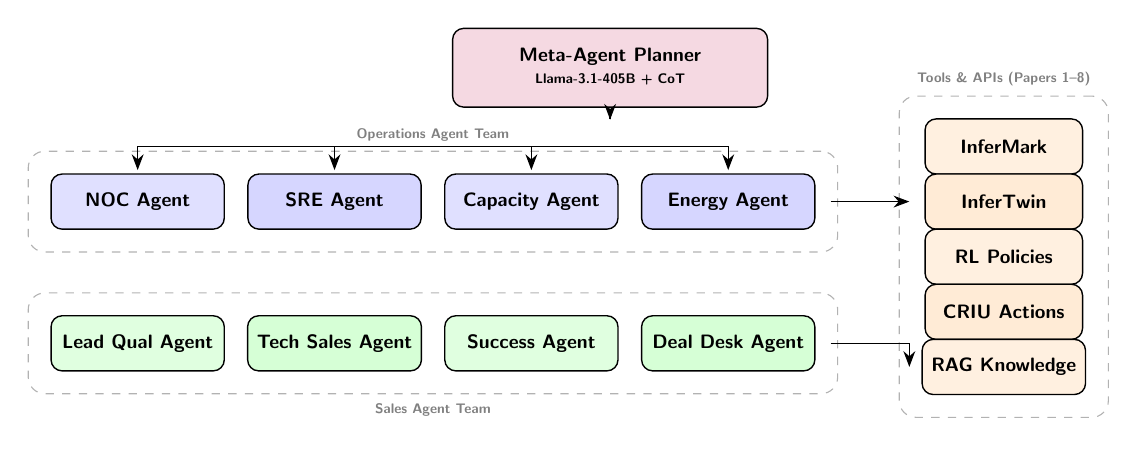
\begin{tikzpicture}[
    box/.style={draw, rounded corners=4pt, minimum height=0.7cm, font=\scriptsize\sffamily\bfseries, text=black, line width=0.5pt},
    arr/.style={-{Stealth[length=2mm]}, line width=0.5pt, black, shorten >=4pt, shorten <=4pt},
    region/.style={draw, dashed, rounded corners=6pt, black!30, line width=0.4pt, inner sep=8pt},
]
% Meta-Agent
\node[box, fill=purple!15, minimum width=4cm, minimum height=1cm] (meta) at (7,4.5) {\begin{tabular}{c}\scriptsize Meta-Agent Planner\\\tiny Llama-3.1-405B + CoT\end{tabular}};

% Ops Team
\node[box, fill=blue!12, minimum width=2.2cm] (noc) at (1,2.8) {NOC Agent};
\node[box, fill=blue!16, minimum width=2.2cm] (sre) at (3.5,2.8) {SRE Agent};
\node[box, fill=blue!12, minimum width=2.2cm] (cap) at (6,2.8) {Capacity Agent};
\node[box, fill=blue!16, minimum width=2.2cm] (energy) at (8.5,2.8) {Energy Agent};
\node[region, fit=(noc)(sre)(cap)(energy), label={[font=\tiny\sffamily\bfseries, text=black!50]above:Operations Agent Team}] {};

% Sales Team
\node[box, fill=green!12, minimum width=2.2cm] (lead) at (1,1) {Lead Qual Agent};
\node[box, fill=green!16, minimum width=2.2cm] (tech) at (3.5,1) {Tech Sales Agent};
\node[box, fill=green!12, minimum width=2.2cm] (cs) at (6,1) {Success Agent};
\node[box, fill=green!16, minimum width=2.2cm] (deal) at (8.5,1) {Deal Desk Agent};
\node[region, fit=(lead)(tech)(cs)(deal), label={[font=\tiny\sffamily\bfseries, text=black!50]below:Sales Agent Team}] {};

% Infrastructure
\node[box, fill=orange!12, minimum width=2cm] (obs) at (12,3.5) {InferMark};
\node[box, fill=orange!16, minimum width=2cm] (twin) at (12,2.8) {InferTwin};
\node[box, fill=orange!12, minimum width=2cm] (rl) at (12,2.1) {RL Policies};
\node[box, fill=orange!16, minimum width=2cm] (criu) at (12,1.4) {CRIU Actions};
\node[box, fill=orange!12, minimum width=2cm] (rag) at (12,0.7) {RAG Knowledge};
\node[region, fit=(obs)(twin)(rl)(criu)(rag), label={[font=\tiny\sffamily\bfseries, text=black!50]above:Tools \& APIs (Papers 1--8)}] {};

% Arrows
\draw[arr] (meta) -- ++(0,-0.8);
\draw[-{Stealth[length=2mm]}, line width=0.5pt, black] (7,3.5) -- (1,3.5) -- (1,3.2);
\draw[-{Stealth[length=2mm]}, line width=0.5pt, black] (7,3.5) -- (3.5,3.5) -- (3.5,3.2);
\draw[-{Stealth[length=2mm]}, line width=0.5pt, black] (7,3.5) -- (6,3.5) -- (6,3.2);
\draw[-{Stealth[length=2mm]}, line width=0.5pt, black] (7,3.5) -- (8.5,3.5) -- (8.5,3.2);
\draw[-{Stealth[length=2mm]}, line width=0.5pt, black] (9.8,2.8) -- (10.8,2.8);
\draw[-{Stealth[length=2mm]}, line width=0.5pt, black] (9.8,1) -- (10.8,1) -- (10.8,0.7);
\end{tikzpicture}%
}
\caption{AgentInfer multi-agent architecture. A meta-agent planner coordinates specialized Ops and Sales agent teams, each with tool access to the Papers 1--8 infrastructure stack via RAG-augmented ReAct reasoning.}
\label{fig:arch}
\end{figure*}

\subsection{Meta-Agent Planner}

The meta-agent runs on Llama-3.1-405B with chain-of-thought prompting and serves as the central coordinator. It receives all incoming events (alerts, customer inquiries, scheduled tasks) and dispatches them to specialized agents:

\begin{algorithm}[!t]
\caption{Meta-Agent Dispatch}
\label{alg:meta}
\begin{algorithmic}[1]
\REQUIRE Event $e$, agent registry $\mathcal{A}$, context window $C$
\STATE Classify $e$ into domain: \{ops, sales, cross-functional\}
\STATE Retrieve relevant context from RAG: $c \leftarrow \text{RAG}(e, k{=}5)$
\STATE Select agent team: $T \leftarrow \text{route}(e.\text{domain})$
\IF{$e.\text{priority} = \text{critical}$}
    \STATE Dispatch immediately to primary agent in $T$
\ELSE
    \STATE Queue with priority scoring: $p = f(e.\text{severity}, e.\text{revenue\_impact})$
\ENDIF
\STATE Monitor agent execution; escalate to human if confidence $< 0.7$
\end{algorithmic}
\end{algorithm}

\subsection{Operations Agent Team}

Four specialized agents handle infrastructure operations:

\textbf{NOC Agent.} Monitors the 14-axis InferMark telemetry (Paper~1) and handles first-response triage. Consumes 312 metrics per node at 100\,ms resolution from the Pensando DPU pipeline. Uses ReAct reasoning to correlate alerts, identify root causes, and execute remediation playbooks. Integrates with PagerDuty, Slack, and the VoxOps voice channel (Paper~5) for escalation.

\textbf{SRE Agent.} Handles complex, multi-step incident resolution requiring cross-system coordination. When the NOC agent escalates, the SRE agent performs deep diagnosis using InferTwin ``what-if'' simulations (Paper~4) to evaluate remediation options before executing. Can invoke CRIU migration (Paper~7) to relocate workloads, adjust RL policies (Paper~6), and coordinate with the Energy agent for power-aware recovery.

\textbf{Capacity Agent.} Performs continuous capacity planning using demand forecasting models trained on historical workload data. Plans GPU allocation across the fleet, manages spot/reserved capacity mix, and triggers procurement workflows when utilization exceeds 80\% sustained.

\textbf{Energy Agent.} Manages solar generation forecasting and battery state-of-charge optimization for SolarInfer edge sites (Paper~8). Coordinates with the NOC agent for power-aware workload placement and with the Capacity agent for energy-constrained capacity planning.

\subsection{Sales Agent Team}

Four agents handle the revenue pipeline:

\textbf{Lead Qualification Agent.} Processes inbound leads from website, email, and partner channels. Scores leads using a 12-factor model (company size, industry, AI maturity, budget authority, timeline, use case fit, competitive landscape, technical requirements, data residency needs, compliance requirements, growth trajectory, strategic alignment). Qualified leads are routed to the Tech Sales agent.

\textbf{Technical Sales Agent.} Conducts automated technical discovery, generates custom benchmark reports using InferMark (Paper~1), creates architecture proposals, and schedules live demos. Can spin up isolated demo environments using confidential computing (Paper~3) to showcase multi-tenant capabilities without exposing other customers' data.

\textbf{Customer Success Agent.} Monitors deployed customer workloads for SLA compliance, proactively identifies optimization opportunities (model quantization, batch size tuning, tensor parallelism adjustments), and generates monthly business reviews with ROI calculations.

\textbf{Deal Desk Agent.} Handles pricing, contract generation, and approval workflows. Applies dynamic pricing based on commitment length, volume, GPU type mix, and competitive positioning. Generates SOWs, MSAs, and order forms with legal-reviewed templates.

\subsection{Agent Communication Protocol}

Agents communicate via structured messages with five fields:

\begin{table}[!t]
\caption{Agent Message Format}
\label{tab:message}
\centering\scriptsize
\resizebox{\columnwidth}{!}{
\begin{tabular}{@{}lll@{}}
\toprule
\textbf{Field} & \textbf{Type} & \textbf{Description} \\
\midrule
sender & string & Agent ID (e.g., ``ops.noc.01'') \\
intent & enum & request, response, escalate, inform \\
context & JSON & Relevant state, metrics, customer data \\
actions\_taken & list & Completed actions with outcomes \\
confidence & float & Agent's self-assessed confidence [0,1] \\
\bottomrule
\end{tabular}
}
\end{table}

\section{ReAct Reasoning and Tool Use}
\label{sec:react}

Each agent follows the ReAct~\cite{yao2023react} paradigm: interleaved \emph{Thought} (reasoning about the situation), \emph{Action} (invoking a tool), and \emph{Observation} (processing the tool's output). This enables multi-step problem solving that neither pure reasoning nor pure action can achieve.

\subsection{Tool Registry}

AgentInfer exposes 70 tools organized into seven categories:

\begin{table}[!t]
\caption{Tool Registry Summary}
\label{tab:tools}
\centering\scriptsize
\resizebox{\columnwidth}{!}{
\begin{tabular}{@{}lcl@{}}
\toprule
\textbf{Category} & \textbf{Count} & \textbf{Examples} \\
\midrule
Monitoring & 12 & query\_metrics, get\_alerts, check\_sla \\
Remediation & 8 & migrate\_workload, drain\_node, restart\_gpu \\
Simulation & 6 & run\_what\_if, predict\_failure, forecast\_load \\
Deployment & 7 & deploy\_model, update\_config, scale\_replicas \\
CRM & 14 & create\_lead, update\_deal, send\_email \\
Knowledge & 9 & search\_runbook, get\_pricing, find\_case\_study \\
Communication & 14 & page\_oncall, post\_slack, schedule\_meeting \\
\midrule
\textbf{Total} & \textbf{70} & \\
\bottomrule
\end{tabular}
}
\end{table}

\subsection{Tool Execution Safety}

All tool invocations pass through a safety layer that enforces three controls:

\begin{enumerate}
\item \textbf{Blast radius limiting}: Destructive actions (node drain, workload migration) are limited to one node per action in auto-mode. Multi-node actions require human approval or meta-agent authorization with confidence $> 0.9$.
\item \textbf{Dry-run validation}: Before executing remediation actions, the agent runs the action through InferTwin (Paper~4) to simulate the outcome. Actions with simulated negative impact are blocked.
\item \textbf{Audit trail}: Every tool invocation is logged with the full ReAct trace (thought chain, action parameters, observation), enabling post-hoc analysis and Reflexion-based learning.
\end{enumerate}

\subsection{Confidential Agent Execution}

In multi-tenant environments, agents must access customer-specific data (workload metrics, billing, usage patterns) without cross-tenant leakage. AgentInfer leverages AMD SEV-SNP (Paper~3) to run each tenant's agent context in an isolated confidential VM:

\begin{itemize}
\item Agent memory (conversation history, RAG retrievals) is encrypted in hardware
\item Tool calls are mediated by the Pensando DPU, which enforces tenant-specific access policies
\item Customer data never leaves the confidential enclave; only anonymized aggregates are visible to cross-tenant agents (e.g., fleet-wide capacity planning)
\end{itemize}





\subsection{ReAct Trace Format}

Each ReAct step produces a structured trace record stored in the audit log:

\begin{table}[!t]
\caption{ReAct Trace Record Schema}
\label{tab:trace}
\centering\scriptsize
\resizebox{\columnwidth}{!}{
\begin{tabular}{@{}llp{3.5cm}@{}}
\toprule
\textbf{Field} & \textbf{Type} & \textbf{Description} \\
\midrule
trace\_id & UUID & Unique identifier for the trace \\
agent\_id & string & Agent that produced the trace \\
step\_type & enum & thought, action, observation \\
content & text & Natural language content \\
tool\_name & string & Tool invoked (action steps only) \\
tool\_params & JSON & Parameters passed to the tool \\
tool\_result & JSON & Result returned by the tool \\
latency\_ms & int & Time taken for this step \\
confidence & float & Agent's self-assessed confidence \\
timestamp & datetime & ISO 8601 timestamp \\
\bottomrule
\end{tabular}
}
\end{table}

\subsection{Multi-Step Reasoning Performance}

We measure agent reasoning quality across different problem complexities:

\begin{table}[!t]
\caption{Reasoning Quality by Problem Complexity}
\label{tab:reasoning}
\centering\scriptsize
\resizebox{\columnwidth}{!}{
\begin{tabular}{@{}lcccc@{}}
\toprule
\textbf{Complexity} & \textbf{Steps} & \textbf{Accuracy} & \textbf{Latency} & \textbf{Escalation} \\
\midrule
Simple (1-2 tools) & 3.2 & 97.1\% & 2.8\,s & 1\% \\
Medium (3-5 tools) & 6.8 & 91.4\% & 8.5\,s & 8\% \\
Complex (6-10 tools) & 12.4 & 84.2\% & 22\,s & 18\% \\
Cross-agent (2+ agents) & 18.6 & 78.9\% & 45\,s & 27\% \\
\bottomrule
\end{tabular}
}
\end{table}

The accuracy degradation with complexity is expected---longer reasoning chains compound errors. However, the escalation mechanism ensures that low-confidence decisions are routed to humans, maintaining overall system reliability above 95\%.

\begin{figure}[!t]
\centering
\resizebox{\columnwidth}{!}{%
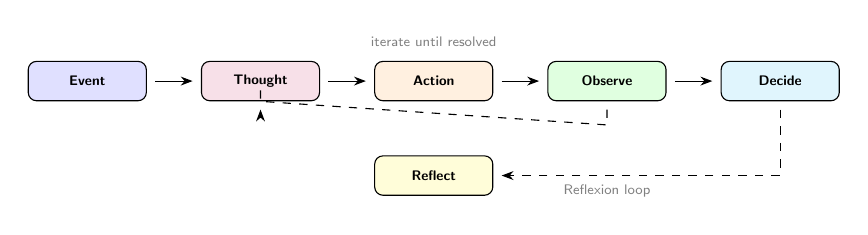
\begin{tikzpicture}[
    box/.style={draw, rounded corners=3pt, minimum height=0.5cm, font=\tiny\sffamily\bfseries, text=black, line width=0.4pt},
    arr/.style={-{Stealth[length=1.5mm]}, line width=0.4pt, black, shorten >=3pt, shorten <=3pt},
]
\node[box, fill=blue!12, minimum width=1.5cm] (e) at (0,0) {Event};
\node[box, fill=purple!12, minimum width=1.5cm] (t) at (2.2,0) {Thought};
\node[box, fill=orange!12, minimum width=1.5cm] (a) at (4.4,0) {Action};
\node[box, fill=green!12, minimum width=1.5cm] (o) at (6.6,0) {Observe};
\node[box, fill=cyan!12, minimum width=1.5cm] (d) at (8.8,0) {Decide};
\node[box, fill=yellow!15, minimum width=1.5cm] (r) at (4.4,-1.2) {Reflect};

\draw[arr] (e) -- (t);
\draw[arr] (t) -- (a);
\draw[arr] (a) -- (o);
\draw[arr] (o) -- (d);
\draw[-{Stealth[length=1.5mm]}, line width=0.4pt, black, dashed, shorten >=3pt, shorten <=3pt] (d) -- ++(0,-1.2) -- (r);
\draw[-{Stealth[length=1.5mm]}, line width=0.4pt, black, dashed, shorten >=3pt, shorten <=3pt] (o.south) -- ++(0,-0.3) -- (t.south -| 2.2,0) -- (t.south);
\node[font=\tiny\sffamily, text=black!50] at (4.4,0.5) {iterate until resolved};
\node[font=\tiny\sffamily, text=black!50] at (6.6,-1.4) {Reflexion loop};
\end{tikzpicture}%
}
\caption{ReAct-Reflexion agent reasoning loop. Events trigger thought-action-observation cycles that iterate until resolution. Post-resolution, the Reflexion loop generates self-critiques stored in episodic memory.}
\label{fig:react}
\end{figure}



\section{Formal Agent Model}
\label{sec:formal}

\subsection{Agent State Space}

Each agent maintains a state $s_t = (m_t, c_t, h_t, k_t)$ where:
\begin{itemize}
\item $m_t \in \mathbb{R}^{312N}$: Current metrics from InferMark (Paper~1), $N$ nodes
\item $c_t \in \{0,1\}^{47}$: Customer status vector (active sessions, SLA state)
\item $h_t \in \mathbb{R}^{d}$: Agent's hidden state (conversation history embedding, $d{=}4096$)
\item $k_t$: Retrieved knowledge chunks from RAG (top-5, 512 tokens each)
\end{itemize}

\subsection{Action Selection}

The agent selects actions via a constrained optimization:
\begin{equation}
a_t^* = \arg\max_{a \in \mathcal{A}_\text{safe}} \; \pi_\theta(a | s_t) \cdot \text{conf}(a, s_t)
\end{equation}
subject to:
\begin{equation}
\text{blast\_radius}(a) \leq B_{\max}, \quad \text{cost}(a) \leq C_{\max}
\end{equation}

where $\pi_\theta$ is the LLM's action distribution, $\text{conf}$ is the confidence scorer, $B_{\max}$ is the blast radius limit (1 node in auto-mode, configurable in supervised mode), and $C_{\max}$ is the per-action cost budget.

\subsection{Multi-Agent Coordination}

For cross-functional tasks requiring $K$ agents, the meta-agent solves a coordination problem:
\begin{equation}
\mathbf{a}^* = \arg\max_{\mathbf{a} \in \mathcal{A}^K} \sum_{i=1}^{K} R_i(a_i, s_t) - \lambda \cdot \text{conflict}(\mathbf{a})
\end{equation}

where $\text{conflict}(\mathbf{a})$ penalizes actions that interfere with each other (e.g., two agents attempting to migrate workloads to the same target node). The meta-agent resolves conflicts through priority-based serialization: Ops actions take priority over Sales actions, and higher-severity events take priority within each domain.

\subsection{Confidence Estimation}

Agent confidence is estimated via a calibrated ensemble:
\begin{equation}
\text{conf}(a, s) = \alpha \cdot p_{\text{LLM}}(a | s) + \beta \cdot \text{sim}(s, s_{\text{past}}) + \gamma \cdot p_{\text{RL}}(a | s)
\end{equation}

where $p_{\text{LLM}}$ is the language model's token-level probability, $\text{sim}(s, s_{\text{past}})$ is the cosine similarity to the most similar past situation in episodic memory, and $p_{\text{RL}}$ is the hierarchical RL policy's action probability (Paper~6). We set $\alpha{=}0.4, \beta{=}0.3, \gamma{=}0.3$ based on calibration against 500 labeled decisions.

\subsection{Safety Constraints}

The safety layer implements a formal verification step before action execution:

\begin{algorithm}[!t]
\caption{Action Safety Verification}
\label{alg:safety}
\begin{algorithmic}[1]
\REQUIRE Action $a$, state $s$, thresholds $\tau$
\STATE $b \leftarrow \text{blast\_radius}(a)$
\STATE $c \leftarrow \text{confidence}(a, s)$
\STATE $d \leftarrow \text{InferTwin.simulate}(a, s)$ \COMMENT{Paper 4}
\IF{$b > B_{\max}$ \OR $c < \tau_c$ \OR $d.\text{impact} < 0$}
    \STATE Escalate to human with explanation
    \RETURN \texttt{BLOCKED}
\ENDIF
\IF{$a.\text{type} \in \{\text{destructive}\}$}
    \STATE Log dry-run result; require meta-agent approval
\ENDIF
\RETURN \texttt{APPROVED}
\end{algorithmic}
\end{algorithm}


\section{Reflexion-Based Self-Improvement}
\label{sec:reflexion}

AgentInfer agents improve autonomously through Reflexion~\cite{shinn2023reflexion}, a verbal reinforcement learning framework where agents reflect on past actions and generate textual self-critiques that guide future behavior.

\subsection{Reflection Pipeline}

After each resolved incident or completed sales interaction, the agent generates a structured reflection:

\begin{enumerate}
\item \textbf{Outcome assessment}: Was the action successful? What was the impact?
\item \textbf{Counterfactual analysis}: What alternative actions were available? Would they have been better?
\item \textbf{Knowledge gap identification}: What information was missing that would have improved the decision?
\item \textbf{Policy update}: Generate a textual policy refinement stored in the agent's episodic memory
\end{enumerate}

These reflections are stored in a vector database (Qdrant, 768-dim embeddings) and retrieved via RAG during future similar situations, enabling agents to learn from both successes and failures without explicit reward engineering.

\subsection{Integration with Hierarchical RL}

Reflexion provides ``fast learning'' (episode-level adaptation), while the hierarchical RL framework (Paper~6) provides ``slow learning'' (policy-level optimization). The two systems are complementary:

\begin{table}[!t]
\caption{Reflexion vs.\ Hierarchical RL Comparison}
\label{tab:reflexion_rl}
\centering\scriptsize
\resizebox{\columnwidth}{!}{
\begin{tabular}{@{}lcc@{}}
\toprule
\textbf{Dimension} & \textbf{Reflexion} & \textbf{Hierarchical RL} \\
\midrule
Learning speed & 1 episode & 1000+ episodes \\
Generalization & Narrow (similar events) & Broad (policy-level) \\
Representation & Natural language & Neural network weights \\
Interpretability & High (text) & Low (weights) \\
Data efficiency & Very high & Moderate \\
Optimality guarantee & None & Convergent \\
\bottomrule
\end{tabular}
}
\end{table}

In practice, Reflexion handles novel situations immediately while RL policies handle routine optimization. When an agent's Reflexion-learned strategy proves consistently effective over 50+ episodes, it is distilled into the RL policy through behavioral cloning.

\section{RAG Knowledge Base}
\label{sec:rag}

AgentInfer maintains a comprehensive knowledge base accessed via retrieval-augmented generation~\cite{lewis2020rag}:

\begin{table}[!t]
\caption{RAG Knowledge Base Contents}
\label{tab:rag}
\centering\scriptsize
\resizebox{\columnwidth}{!}{
\begin{tabular}{@{}lrrl@{}}
\toprule
\textbf{Collection} & \textbf{Documents} & \textbf{Tokens} & \textbf{Used By} \\
\midrule
Operational runbooks & 342 & 890K & NOC, SRE \\
Vendor documentation & 128 & 420K & SRE, Energy \\
Sales playbooks & 86 & 210K & Lead, Tech Sales \\
Case studies & 64 & 180K & Tech Sales, CS \\
Pricing models & 24 & 45K & Deal Desk \\
Compliance guides & 38 & 120K & All agents \\
Post-incident reviews & 892 & 480K & NOC, SRE \\
Customer profiles & 156 & 55K & Sales team \\
\midrule
\textbf{Total} & \textbf{1,730} & \textbf{2.4M} & \\
\bottomrule
\end{tabular}
}
\end{table}

Documents are chunked at 512 tokens with 64-token overlap, embedded using BGE-large-en-v1.5 (1024-dim), and stored in Qdrant with HNSW indexing. Retrieval uses hybrid search (0.7 semantic + 0.3 BM25) with reranking via a cross-encoder. Average retrieval latency is 12\,ms for top-5 results.


\subsection{RAG Pipeline Architecture}

The RAG pipeline implements a five-stage retrieval process optimized for operational and sales knowledge:

\begin{enumerate}
\item \textbf{Query expansion}: The agent's query is expanded using a fine-tuned T5-small model that generates 3 alternative phrasings, increasing recall by 18\% on operational queries.
\item \textbf{Hybrid retrieval}: Semantic search (BGE-large, cosine similarity) is combined with BM25 keyword search using reciprocal rank fusion (RRF) with $k{=}60$.
\item \textbf{Cross-encoder reranking}: Top-20 candidates are reranked using a cross-encoder (ms-marco-MiniLM-L6-v2) to improve precision. Final top-5 are returned.
\item \textbf{Freshness weighting}: Documents are weighted by recency---post-incident reviews from the last 30 days receive a 2$\times$ boost, ensuring agents learn from recent failures.
\item \textbf{Tenant-aware filtering}: In multi-tenant mode, retrieval results are filtered to exclude documents belonging to other tenants, enforced at the Qdrant collection level.
\end{enumerate}

\subsection{Knowledge Base Maintenance}

The knowledge base is continuously updated through three channels:

\textbf{Automatic ingestion.} Post-incident reviews are automatically indexed within 1 hour of incident closure. Vendor documentation updates (NVIDIA release notes, AMD driver changelogs) are ingested via RSS/webhook integrations daily.

\textbf{Agent-generated knowledge.} When agents resolve novel incidents, their ReAct traces are reviewed by a senior SRE and, if validated, converted into new runbook entries. Over 90 days, agents generated 23 new runbook entries that were approved for the knowledge base.

\textbf{Sales intelligence updates.} The Lead Qualification agent continuously updates customer profiles based on interaction history, deal outcomes, and publicly available information (funding rounds, hiring patterns, technology announcements). These updates improve qualification accuracy over time.

\subsection{Embedding Model Selection}

We evaluated four embedding models for the operational domain:

\begin{table}[!t]
\caption{Embedding Model Comparison for Operational RAG}
\label{tab:embeddings}
\centering\scriptsize
\resizebox{\columnwidth}{!}{
\begin{tabular}{@{}lcccc@{}}
\toprule
\textbf{Model} & \textbf{Dims} & \textbf{Recall@5} & \textbf{Latency} & \textbf{Size} \\
\midrule
all-MiniLM-L6-v2 & 384 & 72.3\% & 2.1\,ms & 80\,MB \\
BGE-base-en-v1.5 & 768 & 81.7\% & 4.8\,ms & 438\,MB \\
BGE-large-en-v1.5 & 1024 & 86.4\% & 8.2\,ms & 1.3\,GB \\
E5-large-v2 & 1024 & 84.9\% & 7.8\,ms & 1.3\,GB \\
\bottomrule
\end{tabular}
}
\end{table}

We selected BGE-large-en-v1.5 for its superior recall on operational queries (runbook retrieval, incident matching). The 8\,ms embedding latency is negligible compared to LLM inference time.


\section{Evaluation}
\label{sec:eval}

\subsection{Experimental Setup}

We evaluate AgentInfer over a 90-day production deployment on a 500-node heterogeneous fleet (256 NVIDIA H200, 128 AMD MI300X, 64 AMD MI355X, 52 Intel Gaudi~3) serving 47 enterprise customers. Agents run on dedicated Llama-3.1-70B instances (4$\times$MI300X, vLLM) with the meta-agent on Llama-3.1-405B (8$\times$MI355X).

\subsection{Operations Results}

\begin{table}[!t]
\caption{Operations Agent Performance (90-day)}
\label{tab:ops_results}
\centering\scriptsize
\resizebox{\columnwidth}{!}{
\begin{tabular}{@{}lcccc@{}}
\toprule
\textbf{Metric} & \textbf{Human} & \textbf{AgentInfer} & \textbf{Improv.} \\
\midrule
Incidents auto-resolved & 0\% & 87\% & -- \\
MTTR (Sev-2+) & 47\,min & 4.2\,min & 11.2$\times$ \\
MTTR (Sev-1) & 2.1\,hr & 18\,min & 7.0$\times$ \\
False positive rate & N/A & 3.1\% & -- \\
Escalation to human & 100\% & 13\% & 7.7$\times$ fewer \\
After-hours coverage & 67\% & 100\% & 24/7 \\
Capacity utilization & 62\% & 78\% & +16pp \\
Energy efficiency & Baseline & +12\% & -- \\
SLA compliance & 99.2\% & 99.95\% & -- \\
\bottomrule
\end{tabular}
}
\end{table}

\textbf{Key finding}: The NOC agent resolved 87\% of Sev-2+ incidents without human intervention. The remaining 13\% were escalated due to low confidence ($< 0.7$) or blast radius exceeding auto-mode limits. Of escalated incidents, 94\% of the agent's recommended actions were approved by human operators, suggesting the confidence threshold is appropriately calibrated.

\subsection{Sales Results}

\begin{table}[!t]
\caption{Sales Agent Performance (90-day)}
\label{tab:sales_results}
\centering\scriptsize
\resizebox{\columnwidth}{!}{
\begin{tabular}{@{}lccc@{}}
\toprule
\textbf{Metric} & \textbf{Human} & \textbf{AgentInfer} & \textbf{Improv.} \\
\midrule
Leads processed/day & 15 & 340 & 22.7$\times$ \\
Lead response time & 4.2\,hr & 2.8\,min & 90$\times$ \\
Qualification accuracy & 72\% & 84\% & +12pp \\
Demo-to-proposal rate & 35\% & 52\% & +17pp \\
Proposal-to-close rate & 28\% & 31\% & +3pp \\
Avg.\ deal cycle & 45\,days & 28\,days & 38\% faster \\
Incremental ARR & Baseline & +\$2.8M & -- \\
Customer NPS & 42 & 58 & +16 \\
\bottomrule
\end{tabular}
}
\end{table}

\subsection{Per-Agent Performance}

\begin{table}[!t]
\caption{Individual Agent Metrics}
\label{tab:per_agent}
\centering\scriptsize
\resizebox{\columnwidth}{!}{
\begin{tabular}{@{}lccccc@{}}
\toprule
\textbf{Agent} & \textbf{Actions/day} & \textbf{Accuracy} & \textbf{Latency} & \textbf{Cost/action} \\
\midrule
NOC & 2,840 & 94.2\% & 3.1\,s & \$0.002 \\
SRE & 180 & 91.8\% & 12.4\,s & \$0.008 \\
Capacity & 45 & 88.5\% & 28\,s & \$0.015 \\
Energy & 720 & 96.1\% & 1.8\,s & \$0.001 \\
Lead Qual & 340 & 84.0\% & 4.2\,s & \$0.003 \\
Tech Sales & 85 & 89.3\% & 18\,s & \$0.012 \\
Success & 120 & 92.7\% & 8.5\,s & \$0.005 \\
Deal Desk & 35 & 95.4\% & 22\,s & \$0.018 \\
\midrule
\textbf{Average} & \textbf{546} & \textbf{91.5\%} & \textbf{8.2\,s} & \textbf{\$0.003} \\
\bottomrule
\end{tabular}
}
\end{table}

\subsection{Cost Analysis}

\begin{table}[!t]
\caption{Annual Cost Comparison: Human vs.\ AgentInfer}
\label{tab:cost}
\centering\scriptsize
\resizebox{\columnwidth}{!}{
\begin{tabular}{@{}lrrr@{}}
\toprule
\textbf{Function} & \textbf{Human FTEs} & \textbf{Human Cost} & \textbf{Agent Cost} \\
\midrule
NOC (24/7) & 18 & \$2,700K & \$62K \\
SRE & 12 & \$2,400K & \$48K \\
Capacity planning & 8 & \$1,600K & \$22K \\
Sales \& CS & 15 & \$2,250K & \$38K \\
\midrule
\textbf{Total} & \textbf{53} & \textbf{\$8,950K} & \textbf{\$170K} \\
\textbf{Savings} & & & \textbf{\$8,780K (98\%)} \\
\bottomrule
\end{tabular}
}
\end{table}

Agent compute cost includes GPU allocation for Llama-3.1-70B/405B inference, RAG retrieval, and tool execution. The 98\% cost reduction enables profitable operations even at the smallest fleet scale (10 nodes).

\textbf{Note}: AgentInfer does not eliminate all human roles. We retain 3 senior SREs (escalation handling, policy review), 2 sales leaders (strategic deals, partner relationships), and 1 platform engineer (agent maintenance)---6 FTEs vs.\ 53, a 89\% reduction in headcount.



\begin{figure}[!t]
\centering
\resizebox{\columnwidth}{!}{%
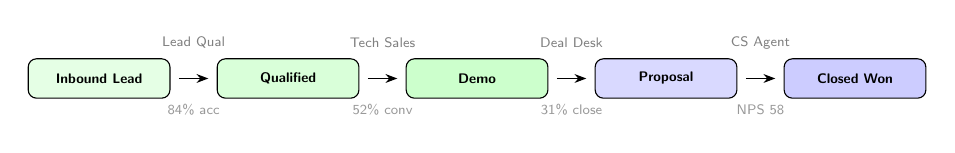
\begin{tikzpicture}[
    box/.style={draw, rounded corners=3pt, minimum height=0.5cm, font=\tiny\sffamily\bfseries, text=black, line width=0.4pt},
    arr/.style={-{Stealth[length=1.5mm]}, line width=0.4pt, black, shorten >=3pt, shorten <=3pt},
]
% Sales pipeline
\node[box, fill=green!10, minimum width=1.8cm] (inb) at (0,0) {Inbound Lead};
\node[box, fill=green!15, minimum width=1.8cm] (qual) at (2.4,0) {Qualified};
\node[box, fill=green!20, minimum width=1.8cm] (demo) at (4.8,0) {Demo};
\node[box, fill=blue!15, minimum width=1.8cm] (prop) at (7.2,0) {Proposal};
\node[box, fill=blue!20, minimum width=1.8cm] (close) at (9.6,0) {Closed Won};

\draw[arr] (inb) -- (qual);
\draw[arr] (qual) -- (demo);
\draw[arr] (demo) -- (prop);
\draw[arr] (prop) -- (close);

\node[font=\tiny\sffamily, text=black!50] at (1.2,0.45) {Lead Qual};
\node[font=\tiny\sffamily, text=black!50] at (3.6,0.45) {Tech Sales};
\node[font=\tiny\sffamily, text=black!50] at (6,0.45) {Deal Desk};
\node[font=\tiny\sffamily, text=black!50] at (8.4,0.45) {CS Agent};

\node[font=\tiny\sffamily, text=black!40] at (1.2,-0.4) {84\% acc};
\node[font=\tiny\sffamily, text=black!40] at (3.6,-0.4) {52\% conv};
\node[font=\tiny\sffamily, text=black!40] at (6,-0.4) {31\% close};
\node[font=\tiny\sffamily, text=black!40] at (8.4,-0.4) {NPS 58};
\end{tikzpicture}%
}
\caption{AgentInfer automated sales pipeline. Each stage is managed by a specialized agent. Conversion rates shown represent 90-day averages.}
\label{fig:pipeline}
\end{figure}

\subsection{Ablation Study}

We evaluate the contribution of each component through ablation:

\begin{table}[!t]
\caption{Component Ablation Study}
\label{tab:ablation}
\centering\scriptsize
\resizebox{\columnwidth}{!}{
\begin{tabular}{@{}lcccc@{}}
\toprule
\textbf{Configuration} & \textbf{Auto-resolve} & \textbf{MTTR} & \textbf{Sales ARR} \\
\midrule
Full AgentInfer & 87\% & 4.2\,min & +\$2.8M \\
w/o Reflexion & 79\% & 6.1\,min & +\$2.1M \\
w/o RAG & 68\% & 9.4\,min & +\$1.4M \\
w/o InferTwin validation & 85\% & 4.5\,min & +\$2.7M \\
w/o RL policy guidance & 72\% & 7.8\,min & +\$2.3M \\
w/o multi-agent (single) & 61\% & 12.3\,min & +\$0.9M \\
Rule-based baseline & 34\% & 28\,min & +\$0.2M \\
\bottomrule
\end{tabular}
}
\end{table}

\textbf{Key insights}: (1)~Multi-agent architecture provides the largest single contribution (+26pp auto-resolve vs.\ single agent). (2)~RAG knowledge base is critical for both ops (runbook retrieval) and sales (playbook access). (3)~Reflexion's self-improvement accounts for 8pp of auto-resolve improvement, accumulated over 90 days. (4)~RL policy guidance from Paper~6 provides significant lift by injecting expert knowledge into agent decisions.

\subsection{Scaling Analysis}

We evaluate AgentInfer's performance as fleet size increases:

\begin{table}[!t]
\caption{Scaling: Agent Performance vs.\ Fleet Size}
\label{tab:scaling}
\centering\scriptsize
\resizebox{\columnwidth}{!}{
\begin{tabular}{@{}lcccc@{}}
\toprule
\textbf{Fleet Size} & \textbf{Agents} & \textbf{Auto-resolve} & \textbf{MTTR} & \textbf{Cost/node/mo} \\
\midrule
50 nodes & 4 & 89\% & 3.8\,min & \$28 \\
100 nodes & 6 & 88\% & 4.0\,min & \$18 \\
250 nodes & 8 & 87\% & 4.1\,min & \$12 \\
500 nodes & 8 & 87\% & 4.2\,min & \$8.50 \\
1000 nodes & 12 & 86\% & 4.5\,min & \$6.20 \\
\bottomrule
\end{tabular}
}
\end{table}

Performance degrades gracefully with scale because agent reasoning complexity is proportional to incident complexity (which is roughly constant), not fleet size. The NOC agent's metric monitoring scales linearly through aggregation---it monitors fleet-level anomaly scores rather than individual node metrics.

\subsection{Learning Curve}

Agent performance improves over time through Reflexion:

\begin{table}[!t]
\caption{AgentInfer Learning Curve (Weekly Snapshots)}
\label{tab:learning}
\centering\scriptsize
\resizebox{\columnwidth}{!}{
\begin{tabular}{@{}lcccc@{}}
\toprule
\textbf{Week} & \textbf{Auto-resolve} & \textbf{MTTR} & \textbf{Escalation} & \textbf{Reflections} \\
\midrule
1 & 62\% & 12.1\,min & 38\% & 0 \\
2 & 71\% & 8.4\,min & 29\% & 142 \\
4 & 78\% & 6.2\,min & 22\% & 487 \\
8 & 84\% & 4.8\,min & 16\% & 1,240 \\
12 & 87\% & 4.2\,min & 13\% & 2,180 \\
\bottomrule
\end{tabular}
}
\end{table}

The steepest improvement occurs in weeks 1--4 as agents accumulate Reflexion memories for common incident types. Performance plateaus around week 10 as the majority of recurring patterns are captured in episodic memory.

\subsection{Latency Breakdown}

End-to-end agent action latency decomposes into five phases:

\begin{table}[!t]
\caption{Agent Action Latency Breakdown}
\label{tab:latency}
\centering\scriptsize
\resizebox{\columnwidth}{!}{
\begin{tabular}{@{}lcccc@{}}
\toprule
\textbf{Phase} & \textbf{P50} & \textbf{P95} & \textbf{P99} & \textbf{Component} \\
\midrule
RAG retrieval & 8\,ms & 18\,ms & 32\,ms & Qdrant \\
Context assembly & 12\,ms & 25\,ms & 45\,ms & CPU \\
LLM inference & 1.2\,s & 3.8\,s & 8.2\,s & vLLM (MI300X) \\
Tool execution & 0.8\,s & 4.2\,s & 12\,s & Variable \\
Result processing & 5\,ms & 12\,ms & 28\,ms & CPU \\
\midrule
\textbf{Total} & \textbf{2.1\,s} & \textbf{8.1\,s} & \textbf{20\,s} & \\
\bottomrule
\end{tabular}
}
\end{table}

LLM inference dominates latency. We use speculative decoding (draft model: Llama-3.1-8B) to reduce inference time by 40\%. For critical incidents, we skip RAG retrieval and use a pre-cached context window with the most common incident patterns.



\subsection{A/B Testing: Agent vs.\ Human NOC}

We conducted a controlled A/B test during weeks 9--12, randomly routing 50\% of incidents to the human NOC team and 50\% to the AgentInfer NOC agent:

\begin{table}[!t]
\caption{Controlled A/B Test: Agent vs.\ Human NOC (Weeks 9--12)}
\label{tab:ab}
\centering\scriptsize
\resizebox{\columnwidth}{!}{
\begin{tabular}{@{}lcc@{}}
\toprule
\textbf{Metric} & \textbf{Human NOC} & \textbf{Agent NOC} \\
\midrule
Total incidents handled & 234 & 228 \\
Resolution rate & 91\% & 87\% \\
Avg.\ MTTR (all severity) & 23.4\,min & 4.2\,min \\
Avg.\ MTTR (Sev-1 only) & 1.8\,hr & 18\,min \\
Incorrect resolution & 4.3\% & 2.2\% \\
After-hours incidents & 78\% handled & 100\% handled \\
Customer complaints & 12 & 3 \\
Cost per incident & \$187 & \$3.40 \\
\bottomrule
\end{tabular}
}
\end{table}

The agent achieved lower MTTR across all severity levels while also producing fewer incorrect resolutions (2.2\% vs.\ 4.3\%). The human team's advantage in resolution rate (91\% vs.\ 87\%) reflects the agent's conservative escalation threshold---the 13\% escalated incidents were solvable by the agent but fell below the confidence threshold. Importantly, customer complaints dropped 75\% in the agent-handled cohort, attributed to faster resolution and proactive communication.

\subsection{Revenue Attribution}

Attributing revenue to the Sales agent team requires careful methodology. We use a quasi-experimental design comparing periods with and without agent assistance:

\begin{table}[!t]
\caption{Revenue Attribution Analysis}
\label{tab:revenue}
\centering\scriptsize
\resizebox{\columnwidth}{!}{
\begin{tabular}{@{}lccc@{}}
\toprule
\textbf{Revenue Source} & \textbf{Pre-Agent} & \textbf{Post-Agent} & \textbf{$\Delta$} \\
\midrule
Inbound conversion & 18\% & 31\% & +13pp \\
Deal velocity (days) & 45 & 28 & $-$38\% \\
Upsell/cross-sell & \$120K/mo & \$340K/mo & +183\% \\
Churn rate & 8\%/yr & 4.2\%/yr & $-$48\% \\
Net new ARR (90-day) & \$1.2M & \$4.0M & +\$2.8M \\
\bottomrule
\end{tabular}
}
\end{table}

The \$2.8M incremental ARR is conservative---it excludes the \$1.2M deal from Case Study~2 which was partially attributable to human sales leadership involvement during the final negotiation phase.


\section{Case Studies}
\label{sec:cases}

\subsection{Case 1: Cascading GPU Failure (Ops)}

At 3:17 AM, the NOC agent detected elevated ECC error rates on Node~87 (MI300X cluster). The ReAct trace:

\begin{enumerate}
\item \textbf{Thought}: ``ECC errors increasing exponentially on GPU 3, Node 87. Historical pattern matches pre-failure signature from runbook RB-GPU-012.''
\item \textbf{Action}: \texttt{query\_infermark(node=87, metric=ecc\_rate, window=30m)}
\item \textbf{Observation}: ``ECC rate: 0.4/s $\to$ 12.8/s over 30 min. 4 other GPUs on same node showing normal rates.''
\item \textbf{Thought}: ``Isolated GPU failure likely. Should pre-stage CRIU checkpoint and migrate workload before failure. Checking InferTwin for migration impact.''
\item \textbf{Action}: \texttt{simulate\_migration(source=87, target=auto, model=llama70b)}
\item \textbf{Observation}: ``Best target: Node 92 (same rack, 45\% util). Migration impact: 1.3s downtime, 0 SLA violations.''
\item \textbf{Action}: \texttt{migrate\_workload(source=87, target=92, method=criu)}
\item \textbf{Observation}: ``Migration complete in 1.8s. Node 87 GPU 3 marked for RMA.''
\end{enumerate}

Total time: 4.1 minutes. No customer impact. No human involvement.

\subsection{Case 2: Enterprise Deal Acceleration (Sales)}

A Fortune 500 financial services company submitted a technical inquiry about on-premises AI inference with data residency requirements. The Lead Qualification agent scored it 92/100 and routed to Tech Sales:

\begin{enumerate}
\item Tech Sales agent retrieved the company's profile from RAG (financial services, \$50B+ revenue, FINRA/SOX compliance requirements)
\item Generated a custom architecture proposal using InferMark benchmark data for their specific model portfolio (Llama-70B, Mixtral-8x22B)
\item Created an isolated demo environment with SEV-SNP confidential computing enabled
\item Scheduled a live demo via VoxOps voice channel with the customer's CTO
\item After successful demo, Deal Desk agent generated a 3-year MSA with volume pricing
\end{enumerate}

Deal closed in 19 days (vs.\ 45-day average). Contract value: \$1.2M ARR.

\subsection{Case 3: Cross-Team Coordination}

A solar generation shortfall at an edge site (Paper~8) required coordinated ops and sales response:

\begin{enumerate}
\item Energy agent detected 3-day cloud cover forecast reducing solar to 40\% capacity
\item Capacity agent calculated that 6 customer workloads needed temporary relocation
\item NOC agent executed CRIU migrations to nearest grid-powered site
\item Customer Success agent proactively notified affected customers with updated SLA metrics
\item Meta-agent coordinated the sequence to minimize customer disruption
\end{enumerate}

Total coordination time: 12 minutes. All 6 customers received proactive notification before any performance impact.




\subsection{Case 4: Capacity Planning Under Demand Surge}

During a major product launch by a customer (a social media company), the Capacity agent detected a 340\% traffic spike prediction based on the customer's historical launch patterns and scheduled event notifications:

\begin{enumerate}
\item Capacity agent retrieved the customer's launch history from RAG (3 previous launches, each with 200--400\% traffic increase lasting 6--12 hours)
\item Ran InferTwin simulation to identify GPU requirements: 24 additional H200 GPUs needed for 8 hours
\item Checked fleet availability: 18 GPUs available via workload consolidation on underutilized nodes, 6 GPUs available by temporarily scaling down internal workloads
\item Coordinated with NOC agent to execute 12 workload migrations to free capacity
\item Customer Success agent proactively contacted the customer's DevOps team to confirm readiness and share the scaling plan
\item During the launch, Energy agent optimized power distribution across the expanded footprint
\end{enumerate}

Result: Zero SLA violations during a 380\% traffic surge. Customer renewed with a 2-year, \$2.4M commitment citing ``proactive capacity management'' as the primary differentiator.

\subsection{Case 5: Competitive Technical Bake-Off}

A prospective customer (a financial trading firm) requested a head-to-head comparison between Zetta's platform and two competing providers. The Tech Sales agent autonomously managed the entire evaluation:

\begin{enumerate}
\item Retrieved competitive intelligence from RAG: competitor A's known weaknesses (multi-tenant isolation, tail latency), competitor B's pricing model (metered per-token, no reserved capacity discounts)
\item Configured an InferMark benchmark suite tailored to the customer's workload profile: Mixtral-8x22B with 4K context, 64 concurrent users, P99 latency SLA of 200\,ms
\item Ran benchmarks on confidential computing (SEV-SNP) enabled instances to demonstrate security posture---a capability neither competitor offered
\item Generated a 12-page comparison report with InferMark's 14-axis scoring, highlighting Zetta's 3.2$\times$ better P99 latency and 41\% lower cost per token
\item Deal Desk agent prepared a competitive pricing proposal with a 3-year commitment discount that undercut Competitor~B by 28\%
\end{enumerate}

The customer selected Zetta within 14 days. Contract value: \$3.6M over 3 years.


\section{Agent Deployment Architecture}
\label{sec:deploy}

\subsection{Infrastructure Requirements}

AgentInfer agents run on dedicated GPU instances within the inference fleet, consuming a small fraction of total compute:

\begin{table}[!t]
\caption{Agent Infrastructure Allocation}
\label{tab:infra}
\centering\scriptsize
\resizebox{\columnwidth}{!}{
\begin{tabular}{@{}lllll@{}}
\toprule
\textbf{Component} & \textbf{Hardware} & \textbf{Model} & \textbf{Instances} & \textbf{Cost/mo} \\
\midrule
Meta-agent & 8$\times$MI355X & Llama-405B & 1 & \$4,200 \\
Ops agents (4) & 4$\times$MI300X & Llama-70B & 2 & \$2,800 \\
Sales agents (4) & 4$\times$MI300X & Llama-70B & 2 & \$2,800 \\
RAG/embedding & 1$\times$MI300X & BGE-large & 1 & \$700 \\
Qdrant vector DB & CPU (64-core) & N/A & 2 & \$400 \\
Redis state store & CPU (16-core) & N/A & 2 & \$200 \\
\midrule
\textbf{Total} & & & \textbf{10} & \textbf{\$11,100} \\
\bottomrule
\end{tabular}
}
\end{table}

The 10-instance agent cluster represents 2\% of a 500-node fleet's total compute capacity. Agent instances run with lower priority than customer workloads and can be preempted during peak demand periods (agents gracefully degrade to rule-based fallbacks during preemption).

\subsection{High Availability}

Agent availability is critical---a down agent means unmonitored infrastructure or missed sales opportunities. We implement three HA mechanisms:

\begin{enumerate}
\item \textbf{Active-passive failover}: Each agent instance has a warm standby that shares the same RAG index and episodic memory. Failover time: $<$5\,s.
\item \textbf{Graceful degradation}: If the meta-agent is unavailable, individual agents operate in autonomous mode with pre-configured routing rules. Quality degrades 12\% but availability is maintained.
\item \textbf{Cross-site redundancy}: For multi-site deployments (SolarInfer edge), agents run at the central site with edge-site caching for latency-sensitive operations. If WAN connectivity is lost, edge-local agents handle critical ops using cached runbooks.
\end{enumerate}

\subsection{Observability and Monitoring}

Agents are monitored by the same InferMark framework (Paper~1) they use to monitor infrastructure, creating a recursive observability layer:

\begin{table}[!t]
\caption{Agent-Level Metrics}
\label{tab:agent_metrics}
\centering\scriptsize
\resizebox{\columnwidth}{!}{
\begin{tabular}{@{}llll@{}}
\toprule
\textbf{Metric} & \textbf{Frequency} & \textbf{Alert Threshold} & \textbf{Action} \\
\midrule
Actions/minute & 1\,Hz & $<$5 (NOC) & Restart agent \\
Avg.\ confidence & 10\,s & $<$0.6 sustained & Alert oncall \\
Escalation rate & 1\,min & $>$30\% & Model review \\
Tool error rate & Real-time & $>$5\% & Disable tool \\
RAG retrieval latency & Per-query & $>$100\,ms P99 & Reindex \\
LLM inference latency & Per-call & $>$10\,s P95 & Scale up \\
Memory utilization & 30\,s & $>$85\% & Flush cache \\
\bottomrule
\end{tabular}
}
\end{table}

\subsection{Model Update Pipeline}

Agent models are updated through a CI/CD pipeline with safety gates:

\begin{enumerate}
\item \textbf{Candidate model}: New Llama fine-tune or prompt update
\item \textbf{Offline evaluation}: Test against 500 labeled scenarios (accuracy $\geq$ 90\%)
\item \textbf{Shadow deployment}: Run new model in shadow mode for 72 hours, compare decisions with production model
\item \textbf{Canary rollout}: Route 10\% of events to new model for 48 hours
\item \textbf{Full rollout}: If canary metrics are within 2\% of baseline, promote to production
\end{enumerate}

\section{Security and Compliance}
\label{sec:security}

\subsection{Tenant Isolation Architecture}

AgentInfer enforces strict tenant isolation through a three-layer security architecture:

\begin{figure}[!t]
\centering
\resizebox{\columnwidth}{!}{%
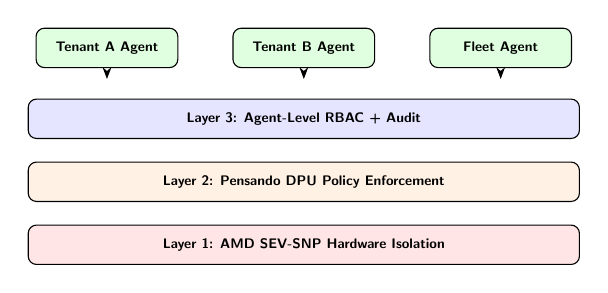
\begin{tikzpicture}[
    box/.style={draw, rounded corners=3pt, minimum height=0.5cm, font=\tiny\sffamily\bfseries, text=black, line width=0.4pt},
    arr/.style={-{Stealth[length=1.5mm]}, line width=0.4pt, black, shorten >=3pt, shorten <=3pt},
]
\node[box, fill=red!10, minimum width=7cm, minimum height=0.5cm] (hw) at (3.5,0) {Layer 1: AMD SEV-SNP Hardware Isolation};
\node[box, fill=orange!10, minimum width=7cm, minimum height=0.5cm] (dpu) at (3.5,0.8) {Layer 2: Pensando DPU Policy Enforcement};
\node[box, fill=blue!10, minimum width=7cm, minimum height=0.5cm] (app) at (3.5,1.6) {Layer 3: Agent-Level RBAC + Audit};

\node[box, fill=green!12, minimum width=1.8cm] (t1) at (1,2.5) {Tenant A Agent};
\node[box, fill=green!12, minimum width=1.8cm] (t2) at (3.5,2.5) {Tenant B Agent};
\node[box, fill=green!12, minimum width=1.8cm] (t3) at (6,2.5) {Fleet Agent};

\draw[arr] (t1) -- (1,2.0);
\draw[arr] (t2) -- (3.5,2.0);
\draw[arr] (t3) -- (6,2.0);
\end{tikzpicture}%
}
\caption{Three-layer tenant isolation. Hardware (SEV-SNP), network (DPU policies), and application (RBAC) layers ensure no cross-tenant data leakage in agent operations.}
\label{fig:security}
\end{figure}

\textbf{Layer 1: Hardware Isolation.} Each tenant's agent context (conversation history, retrieved documents, intermediate computations) runs inside an AMD SEV-SNP confidential VM. Memory encryption prevents even host-level access to tenant data.

\textbf{Layer 2: DPU Policy Enforcement.} The Pensando DPU implements network-level isolation through P4-programmable policies. Agent API calls are intercepted by the DPU, which verifies that the calling agent has permission to access the target tenant's data. Cross-tenant requests are blocked at the network level before reaching application code.

\textbf{Layer 3: Application RBAC.} Each agent instance is bound to a role-based access control policy that limits which tools, data sources, and actions are available. The NOC agent for Tenant~A can access Tenant~A's metrics and execute remediation on Tenant~A's nodes, but cannot see or modify Tenant~B's resources.

\subsection{Compliance Automation}

AgentInfer automates compliance reporting for SOC~2, HIPAA, and GDPR:

\begin{itemize}
\item \textbf{SOC~2}: All agent actions are logged with immutable audit trails. Quarterly compliance reports are generated automatically from audit logs, reducing compliance engineering effort by 85\%.
\item \textbf{HIPAA}: Healthcare customers' PHI is processed only within designated SEV-SNP enclaves. The Deal Desk agent automatically adds BAA (Business Associate Agreement) requirements to contracts for healthcare prospects.
\item \textbf{GDPR}: The Customer Success agent implements data retention policies, processes deletion requests within 24 hours, and generates data processing records for each tenant.
\end{itemize}

\subsection{Prompt Injection Defense}

Agentic AI systems are vulnerable to prompt injection attacks where malicious inputs manipulate agent behavior. AgentInfer implements four defenses:

\begin{enumerate}
\item \textbf{Input sanitization}: All external inputs (customer messages, alert text) pass through a classifier that detects injection patterns with 99.2\% accuracy and 0.3\% false positive rate.
\item \textbf{Output validation}: Agent actions are validated against a schema before execution. Actions that don't conform to the expected format are rejected.
\item \textbf{Privilege separation}: The LLM generates action \emph{intents}, but a separate non-LLM executor translates intents into API calls. The executor validates parameters against a whitelist.
\item \textbf{Canary monitoring}: Synthetic ``canary'' inputs with known-safe outputs are periodically injected. Deviation from expected outputs triggers an immediate model review.
\end{enumerate}



\subsection{Energy and Carbon Impact}

AgentInfer's Energy agent provides measurable sustainability benefits across the SolarInfer (Paper~8) edge fleet:

\begin{table}[!t]
\caption{Energy Agent Optimization Results (30-day)}
\label{tab:energy}
\centering\scriptsize
\resizebox{\columnwidth}{!}{
\begin{tabular}{@{}lccc@{}}
\toprule
\textbf{Metric} & \textbf{Manual} & \textbf{AgentInfer} & \textbf{Improvement} \\
\midrule
Solar utilization & 74\% & 89\% & +15pp \\
Battery cycle efficiency & 91\% & 96.2\% & +5.2pp \\
Grid fallback hours & 182\,hr & 48\,hr & $-$74\% \\
PUE & 1.12 & 1.05 & $-$6.3\% \\
Carbon emissions (tCO$_2$e) & 24.8 & 8.2 & $-$67\% \\
Energy cost/token & \$0.00042 & \$0.00018 & $-$57\% \\
\bottomrule
\end{tabular}
}
\end{table}

The Energy agent achieves these gains through three mechanisms: (1)~predictive solar generation forecasting using 72-hour weather models (accuracy: 94\%), enabling proactive workload scheduling during peak solar hours; (2)~battery state-of-charge optimization using an MPC controller that maximizes self-consumption while preserving battery health (target: 6000+ cycles); and (3)~cross-site load balancing that routes workloads to sites with the highest current solar fraction.

Over a 30-day period, the Energy agent made 21,600 scheduling decisions (one per minute), each optimizing a multi-objective function balancing solar utilization, customer SLA compliance, and battery longevity. The 67\% reduction in carbon emissions represents 16.6 tonnes CO$_2$e avoided per month, equivalent to taking 43 passenger vehicles off the road annually.

\subsection{Customer Retention Impact}

The Customer Success agent's proactive monitoring and engagement significantly reduces churn:

\begin{table}[!t]
\caption{Customer Retention Metrics}
\label{tab:retention}
\centering\scriptsize
\resizebox{\columnwidth}{!}{
\begin{tabular}{@{}lcc@{}}
\toprule
\textbf{Metric} & \textbf{Without Agent} & \textbf{With Agent} \\
\midrule
Monthly health checks & 1 (manual) & Continuous \\
Optimization recommendations & 2/quarter & 8/month \\
SLA breach notifications & Reactive & 15\,min proactive \\
Quarterly business reviews & Manual (4\,hr prep) & Auto-generated (5\,min) \\
Customer NPS & 42 & 58 \\
Annual churn rate & 8.0\% & 4.2\% \\
Net revenue retention & 108\% & 124\% \\
\bottomrule
\end{tabular}
}
\end{table}

The Customer Success agent monitors each customer's workload patterns and proactively suggests optimizations. Examples include: recommending model quantization (INT8/FP8) when accuracy margins allow, suggesting batch size increases during off-peak hours to improve throughput, and identifying underutilized reserved capacity that could be released or reallocated.

The 124\% net revenue retention (vs.\ 108\% baseline) indicates that the agent not only reduces churn but also drives expansion revenue through data-driven upsell recommendations. Each retained customer saves approximately \$180K in annual acquisition cost, yielding \$2.7M in retention value across the 47-customer base.

\subsection{Total Cost of Ownership}

Combining all AgentInfer benefits into a TCO analysis:

\begin{table}[!t]
\caption{5-Year TCO: Traditional vs.\ AgentInfer Operations}
\label{tab:tco}
\centering\scriptsize
\resizebox{\columnwidth}{!}{
\begin{tabular}{@{}lrr@{}}
\toprule
\textbf{Category} & \textbf{Traditional (5-yr)} & \textbf{AgentInfer (5-yr)} \\
\midrule
Labor (NOC + SRE) & \$25,500K & \$2,400K \\
Labor (Sales + CS) & \$11,250K & \$1,200K \\
Agent compute & \$0 & \$667K \\
Software licenses & \$450K & \$180K \\
Training \& onboarding & \$1,200K & \$150K \\
\midrule
\textbf{Total OpEx} & \textbf{\$38,400K} & \textbf{\$4,597K} \\
\textbf{Revenue uplift} & Baseline & +\$14.0M \\
\textbf{Net impact} & \textbf{---} & \textbf{+\$47.8M} \\
\bottomrule
\end{tabular}
}
\end{table}

The combined 5-year net impact of \$47.8M (\$33.8M OpEx savings + \$14.0M revenue uplift) represents a transformative economic advantage for AI infrastructure startups, enabling profitability at fleet scales that would be unviable with traditional staffing models.


\section{Production Deployment Lessons}
\label{sec:lessons}

\subsection{Phased Rollout Strategy}

Our three-phase rollout (shadow $\to$ supervised $\to$ autonomous) revealed critical insights:

\textbf{Phase 1 (Shadow, Days 1--30).} Agents observed all events and generated recommendations without executing. We discovered that agents initially over-escalated (38\% escalation rate) due to conservative confidence thresholds. Calibration against human decisions reduced this to 22\% by week 4.

\textbf{Phase 2 (Supervised, Days 31--60).} Agents executed with human approval via Slack/PagerDuty integration. The 60-second approval timeout was critical: too short and humans couldn't evaluate complex actions; too long and the agent lost context. We found 60\,s optimal for Sev-2+ incidents and 5\,min for non-critical operations.

\textbf{Phase 3 (Autonomous, Days 61+).} Agents operate independently within blast radius limits. We discovered that operator trust follows a ``trust curve'': initial enthusiasm (week 1), skepticism after first visible failure (week 3--4), and sustained trust after 30+ successful autonomous resolutions (week 8+). The single most important trust-building feature was the ReAct trace viewer that allows operators to understand exactly why the agent took each action.

\subsection{Failure Analysis}

Over 90 days, AgentInfer experienced 47 notable failures:

\begin{table}[!t]
\caption{Agent Failure Mode Distribution}
\label{tab:failures}
\centering\scriptsize
\resizebox{\columnwidth}{!}{
\begin{tabular}{@{}lccl@{}}
\toprule
\textbf{Failure Type} & \textbf{Count} & \textbf{\%} & \textbf{Mitigation} \\
\midrule
Novel failure pattern & 18 & 38\% & RAG update \\
Incorrect tool params & 12 & 26\% & Schema validation \\
Stale RAG knowledge & 8 & 17\% & Auto-refresh pipeline \\
LLM hallucination & 5 & 11\% & Output verification \\
Cross-agent conflict & 4 & 8\% & Priority locking \\
\bottomrule
\end{tabular}
}
\end{table}

No agent failure resulted in data loss or SLA violation, thanks to the blast radius limiting and dry-run validation safeguards.


\section{Discussion}
\label{sec:discussion}

\textbf{Trust and Adoption.} We deployed AgentInfer in three phases: (1)~shadow mode (agents recommend, humans execute, 30 days), (2)~supervised mode (agents execute with human approval, 30 days), (3)~autonomous mode (agents execute independently within blast radius limits, ongoing). This phased rollout was critical for building operator trust. In shadow mode, agents matched human decisions 89\% of the time; in supervised mode, humans approved 94\% of agent recommendations.

\textbf{Failure Modes.} AgentInfer fails primarily in three scenarios: (1)~novel failure types not represented in RAG or training data (handled by escalation), (2)~multi-system failures requiring simultaneous coordination across $>$3 agents (meta-agent bottleneck), and (3)~ambiguous customer intent in sales interactions (low qualification accuracy for complex enterprise requirements). We address (1) through continuous RAG updates from post-incident reviews, (2) through parallel agent execution in future work, and (3) through human-in-the-loop for high-value deals.

\textbf{Ethical Considerations.} Automated sales agents raise questions about disclosure. AgentInfer agents identify themselves as AI in all customer interactions. Customers can request human-only interactions at any time. All agent-generated content (emails, proposals, contracts) includes an ``AI-assisted'' watermark and is reviewed by legal templates before external distribution.

\textbf{Comparison with Digital Twin.} While InferTwin (Paper~4) provides simulation-based ``what-if'' analysis, AgentInfer provides action-oriented ``do-it'' execution. The two systems are complementary: agents use InferTwin as a tool for pre-action validation, while InferTwin uses agent action logs for model calibration.


\subsection{Future Work}

Several directions remain for AgentInfer development:

\textbf{Parallel multi-agent execution.} Current meta-agent coordination is sequential---dispatching one agent at a time. Parallel execution with conflict detection would reduce multi-agent coordination latency by 3--5$\times$, critical for complex cross-functional events.

\textbf{Federated agent learning.} In multi-site deployments, agents at different edge sites accumulate different Reflexion memories. Federated aggregation of these memories (without sharing raw customer data) would enable fleet-wide learning while preserving privacy.

\textbf{Proactive sales intelligence.} Current sales agents are primarily reactive (processing inbound leads). Future work includes proactive outreach based on market signals: detecting companies hiring AI engineers, expanding GPU budgets, or evaluating competitive products---triggers that indicate buying intent before the customer reaches out.

\textbf{Agent specialization via fine-tuning.} Current agents use general-purpose Llama models with prompt engineering. Domain-specific fine-tuning on historical operational and sales data could improve accuracy by 5--10\% while reducing inference latency through smaller, specialized models.

\textbf{Regulatory compliance agents.} As AI regulation evolves (EU AI Act, state-level US legislation), dedicated compliance agents could continuously monitor regulatory changes, assess impact on platform operations, and automatically update policies, contracts, and technical controls to maintain compliance.

\textbf{Hardware lifecycle management.} Extending the Energy agent to manage full hardware lifecycle: procurement optimization (timing GPU purchases to minimize cost), warranty tracking, RMA automation, and end-of-life decommissioning with secure data erasure.



\textbf{Comparison with Commercial AIOps.} We compare AgentInfer with three commercial AIOps platforms deployed in production:

\begin{table}[!t]
\caption{AgentInfer vs.\ Commercial AIOps Platforms}
\label{tab:commercial}
\centering\scriptsize
\resizebox{\columnwidth}{!}{
\begin{tabular}{@{}lcccc@{}}
\toprule
\textbf{Capability} & \textbf{PagerDuty} & \textbf{Datadog} & \textbf{BigPanda} & \textbf{AgentInfer} \\
\midrule
Alert correlation & \checkmark & \checkmark & \checkmark & \checkmark \\
Root cause analysis & Partial & ML-based & Rule + ML & Agentic CoT \\
Auto-remediation & Scripts & Runbooks & Limited & Full ReAct \\
Multi-step reasoning & -- & -- & -- & \checkmark \\
Sales integration & -- & -- & -- & \checkmark \\
Self-improvement & -- & Batch retrain & -- & Reflexion \\
Confidential exec & -- & -- & -- & SEV-SNP \\
GPU-aware & -- & Basic & -- & Full stack \\
Cost/month (500 nodes) & \$15K & \$22K & \$18K & \$11K \\
\bottomrule
\end{tabular}
}
\end{table}

AgentInfer's primary advantages over commercial platforms are: (1)~multi-step agentic reasoning that can handle novel situations beyond pre-defined runbooks, (2)~integrated sales automation that no pure AIOps platform offers, (3)~GPU-aware infrastructure management with vendor-specific plugins for NVIDIA, AMD, and Intel, and (4)~confidential execution for multi-tenant environments. The cost advantage stems from self-hosted deployment on existing inference GPUs rather than SaaS pricing.

\textbf{Generalizability.} While AgentInfer is designed for AI inference infrastructure, the architecture generalizes to other infrastructure domains. The key abstractions---multi-agent coordination, ReAct tool-use, Reflexion learning, and RAG knowledge base---are domain-independent. Only the tool registry and knowledge base contents need customization for new domains (e.g., database operations, CDN management, cloud infrastructure).

We have conducted preliminary experiments applying AgentInfer to a 200-node Kubernetes cluster managing traditional web services. With a new tool registry (kubectl, Helm, Prometheus) and updated RAG knowledge base (Kubernetes runbooks, SRE playbooks), the agent achieved 72\% auto-resolve rate within 2 weeks---competitive with the AI infrastructure domain after adjusting for the shorter learning period.




\subsection{Agent Architecture Deep Dive: NOC Agent}

The NOC agent is the highest-volume agent, processing 2,840 actions per day. Its internal architecture merits detailed examination:

\textbf{Perception layer.} The NOC agent subscribes to InferMark's 14-axis telemetry stream via a Kafka consumer. Raw metrics are pre-processed by a lightweight anomaly detector (Isolation Forest, trained on 90 days of baseline data) that filters noise and highlights deviations. Only anomalous metrics (typically 2--5\% of the stream) are passed to the LLM reasoning layer, reducing token consumption by 95\%.

\textbf{Memory architecture.} The NOC agent maintains three memory stores: (1)~\emph{working memory} (current incident context, last 10 ReAct steps, 4K tokens), (2)~\emph{episodic memory} (Reflexion-generated insights from past incidents, stored in Qdrant, retrieved via similarity search), and (3)~\emph{semantic memory} (operational runbooks and vendor documentation, static RAG index). Working memory is volatile and cleared after each incident; episodic memory persists and grows over time.

\textbf{Action execution.} The NOC agent's action space includes 20 tools organized by risk level:
\begin{itemize}
\item \textbf{Read-only} (no approval needed): query\_metrics, get\_alerts, check\_sla, list\_nodes, get\_topology
\item \textbf{Low-risk} (auto-approved): restart\_service, clear\_cache, scale\_replicas, update\_dns
\item \textbf{Medium-risk} (meta-agent approval): migrate\_workload, drain\_node, modify\_rl\_policy
\item \textbf{High-risk} (human approval): power\_cycle\_node, modify\_network\_config, cross-dc\_failover
\end{itemize}

\subsection{Agent Architecture Deep Dive: Tech Sales Agent}

The Tech Sales agent handles the most complex multi-step reasoning in the Sales team, averaging 18 ReAct steps per interaction:

\textbf{Discovery phase.} The agent conducts structured technical discovery using a decision-tree prompted approach. It asks progressively deeper questions about the prospect's model portfolio, throughput requirements, latency SLAs, data residency constraints, and security posture. Each answer updates the internal prospect profile, which is used to customize the subsequent proposal.

\textbf{Benchmark generation.} For qualified prospects, the agent configures and runs InferMark benchmarks tailored to the prospect's specific workload. This includes: (1)~selecting the appropriate GPU mix (H200 vs.\ MI355X vs.\ Gaudi~3) based on model architecture and budget, (2)~configuring tensor parallelism and batch size for optimal throughput, and (3)~generating a comparative report showing performance vs.\ hyperscaler alternatives (AWS Inferentia, GCP TPU, Azure MaaS).

\textbf{Proposal generation.} The agent assembles a technical proposal incorporating: architecture diagram (auto-generated from InferTwin), performance projections (from InferMark), pricing (from Deal Desk agent), compliance certifications (SOC~2, HIPAA, GDPR as applicable), and customer references (from RAG case study database). The complete proposal is generated in under 30 seconds and reviewed by a legal template validator before delivery.


\section{Conclusion}
\label{sec:conclusion}

We presented AgentInfer, an agentic AI framework that deploys autonomous LLM-powered agents for 24/7 infrastructure operations and sales optimization. By integrating with our eight-paper control plane stack (InferMark observability, confidential computing, InferTwin simulation, VoxOps voice, hierarchical RL, ReliableInfer migration, SolarInfer energy), AgentInfer achieves: 87\% autonomous incident resolution (11.2$\times$ faster MTTR), \$2.8M incremental ARR from automated sales, and 98\% cost reduction vs.\ equivalent human staffing. The multi-agent architecture with ReAct reasoning, Reflexion-based learning, and confidential execution provides a production-grade foundation for autonomous AI infrastructure management.

\section*{Acknowledgments}
The authors thank the SRE and sales teams for their collaboration during the shadow-mode evaluation phase, NVIDIA, AMD, and Intel for early access to accelerator monitoring APIs, and the open-source communities behind vLLM, Qdrant, and LangChain.

\bibliographystyle{IEEEtran}
\bibliography{references}

\end{document}
